\documentclass[12pt, letterpaper]{article}
\usepackage[margin=2.5cm]{geometry}
\usepackage{times}
\usepackage{graphicx}
\usepackage[utf8]{inputenc}
\usepackage[T1]{fontenc}
\usepackage{lmodern}
\usepackage[table,xcdraw]{xcolor}
%%%%%%%%%%%%%%%%%%%%%%%%%%%%%%%%%%%%%%%%%%%%%%%%%%%%
\begin{document}
% title
\fontfamily{ptm}
\title{ENSC 351 - Lab 3: MapReduce}
\date{October 17, 2018}
\author{Nic Klaassen, Galen Elfert, Diane Wolf}
\maketitle
% text
\section{Explanation of workload}
	The workload invented to fit the MapReduce framework better than word counts was {[matrix multiplication | distributed sort problem | merge sort problem]...}
\subsection{Conception}
	{[Matrix multiplication | distributed sort problem | merge sort problem]} was chosen as a better alternative to word counts because...
\subsection{Speed: Single-threaded implementation}
	
\subsection{Speed: MapReduce implementation}
\subsection{Comparison}
\section{Word count efficiency}
	Both implementations of the program counted the instances of words in fifty paragraphs (with a total length of 2261 words) of Lorem Ipsum. They were run on the same machine with hardware to support twelve threads. Ten executions of each implementation were conducted, with the duration measured by the built-in Linux \texttt{time} command. A call graph for both implementations was generated using Valgrind's Callgrind tool.
\subsection{Single-threaded implementation}
	The single-threaded implementation of the word count ran for a mean wall time of 0.0140 seconds. Table 1 below shows the execution time, as well as CPU usage, for each of the ten single-threaded word count runs.\newline
	
	See Figure 2 for a graphical representation of the call map.

	\begin{table}[h]
	\centering
	\begin{tabular}{ccccc}
	\rowcolor[HTML]{FFFFC7} 
	\multicolumn{5}{c}{\cellcolor[HTML]{FFFFC7}\textbf{Execution times for single-threaded word count}} \\
	\rowcolor[HTML]{EFEFEF} 
	run \# & user (s) & system (s) & wall (s) & CPU usage (\%) \\
	1 & 0 & 0.004 & 0 & 0 \\
	2 & 0 & 0.008 & 0.01 & 0 \\
	3 & 0.004 & 0 & 0.02 & 0 \\
	4 & 0 & 0.004 & 0.01 & 0 \\
	5 & 0 & 0.004 & 0.01 & 0 \\
	6 & 0.004 & 0 & 0.01 & 0 \\
	7 & 0 & 0.004 & 0.02 & 0 \\
	8 & 0.004 & 0 & 0.01 & 0 \\
	9 & 0.004 & 0 & 0.04 & 0 \\
	10 & 0 & 0.004 & 0.01 & 0 \\
	\rowcolor[HTML]{D0F0D0} 
	\multicolumn{1}{r}{\cellcolor[HTML]{9AFF99}mean (s)} & 0.0016 & 0.0028 & 0.0140 & 0 \\
	\rowcolor[HTML]{ECF4FF} 
	\multicolumn{1}{r}{\cellcolor[HTML]{DAE8FC}std. dev. (s)} & 0.0021 & 0.0027 & 0.0107 & 0
	\end{tabular}
	\caption{Duration of single-threaded implementation measured by \texttt{time}}
	\end{table}
\subsection{MapReduce implementation}
	The MapReduce implementation of the word count was tested with four threads and then the full twelve threads the machine was capable of supporting. Tables 2 and 3 below show the execution time, as well as CPU usage, for each of the ten word counts run with MapReduce. Note that the greater the quantity of threads used to multithread, the slower the program execution became. As the thread count increased, the CPU usage also appeared to increase, going from an average of 10\% with four threads to an average of 40\% with 12 threads.\newline

	See Figure 2 for a graphical representation of the call map.

	\begin{table}[h]
	\centering
	\begin{tabular}{ccccc}
	\multicolumn{5}{c}{\cellcolor[HTML]{FFFFC7}\textbf{Execution times for MapReduce word count - 4 threads}} \\
	\cellcolor[HTML]{EFEFEF}run \# & \cellcolor[HTML]{EFEFEF}user (s) & \cellcolor[HTML]{EFEFEF}system (s) & 				\cellcolor[HTML]{EFEFEF}wall (s) & \cellcolor[HTML]{EFEFEF}CPU usage (\%) \\
	1 & 0.008 & 0 & 0.02 & 0 \\
	2 & 0.008 & 0 & 0.03 & 0 \\
	3 & 0.008 & 0 & 0.02 & 0 \\
	4 & 0.008 & 0 & 0.02 & 0 \\
	5 & 0.008 & 0 & 0.01 & 0 \\
	6 & 0.008 & 0 & 0.02 & 0 \\
	7 & 0.008 & 0 & 0.01 & 0 \\
	8 & 0.008 & 0 & 0.02 & 0 \\
	9 & 0.008 & 0 & 0.03 & 0 \\
	10 & 0.012 & 0 & 0.01 & 100 \\
	\rowcolor[HTML]{D0F0D0} 
	\multicolumn{1}{r}{\cellcolor[HTML]{9AFF99}mean (s)} & 0.0084 & 0 & 0.0190 & 10.0000 \\
	\rowcolor[HTML]{ECF4FF} 
	\multicolumn{1}{r}{\cellcolor[HTML]{DAE8FC}std. dev. (s)} & 0.0013 & 0 & 0.0074 & 31.6228
	\end{tabular}
	\caption{Duration of MapReduce implementation measured by \texttt{time}, with four threads}
	\end{table}

	\begin{table}[h]
	\centering
	\begin{tabular}{ccccc}
	\multicolumn{5}{c}{\cellcolor[HTML]{FFFFC7}\textbf{Execution times for MapReduce word count - 12 threads}} \\
	\rowcolor[HTML]{EFEFEF} 
	run \# & user (s) & system (s) & wall (s) & CPU usage (\%) \\
	1 & 0.008 & 0.004 & 0.01 & 0 \\
	2 & 0.008 & 0.008 & 0.03 & 0 \\
	3 & 0.008 & 0.008 & 0.01 & 0 \\
	4 & 0.008 & 0.004 & 0.01 & 0 \\
	5 & 0.016 & 0 & 0.01 & 100 \\
	6 & 0.008 & 0.004 & 0.01 & 0 \\
	7 & 0.012 & 0.004 & 0.01 & 100 \\
	8 & 0.008 & 0.008 & 0.01 & 0 \\
	9 & 0.012 & 0 & 0.01 & 100 \\
	10 & 0.016 & 0 & 0.01 & 100 \\
	\rowcolor[HTML]{D0F0D0} 
	\multicolumn{1}{r}{\cellcolor[HTML]{9AFF99}mean (s)} & 0.0104 & 0.0040 & 0.0120 & 40.0000 \\
	\rowcolor[HTML]{ECF4FF} 
	\multicolumn{1}{r}{\cellcolor[HTML]{DAE8FC}std. dev. (s)} & 0.0034 & 0.0033 & 0.0063 & 51.6398
	\end{tabular}
	\caption{Duration of MapReduce implementation measured by \texttt{time}, with twelve threads}
	\end{table}
\subsection{Comparison}
	
\section{Most appropriate workload for MapReduce}
	Data that needs sorting?
\section{Impact of using multiple machines on execution speed}
	
\newpage
	\begin{figure}[h]
	\centering
	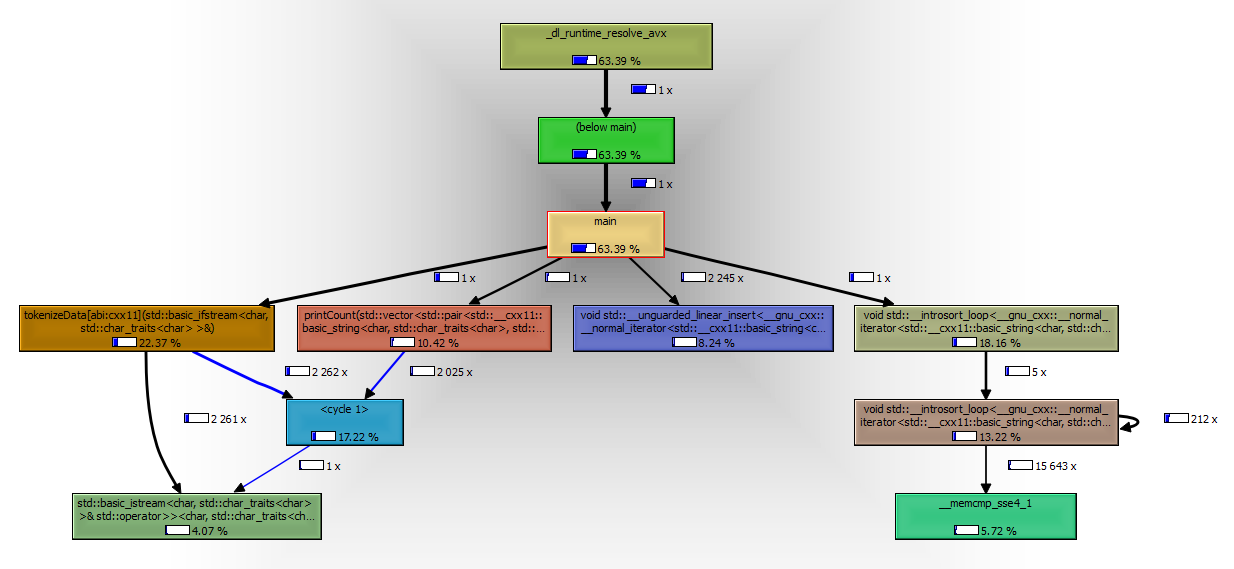
\includegraphics[width=1.35\textwidth, angle=90]{call-graph-part3-cropped}
	\caption{Call map for single-threaded implementation of word count}
	\end{figure}
\newpage
	\begin{figure}[h]
	\centering
	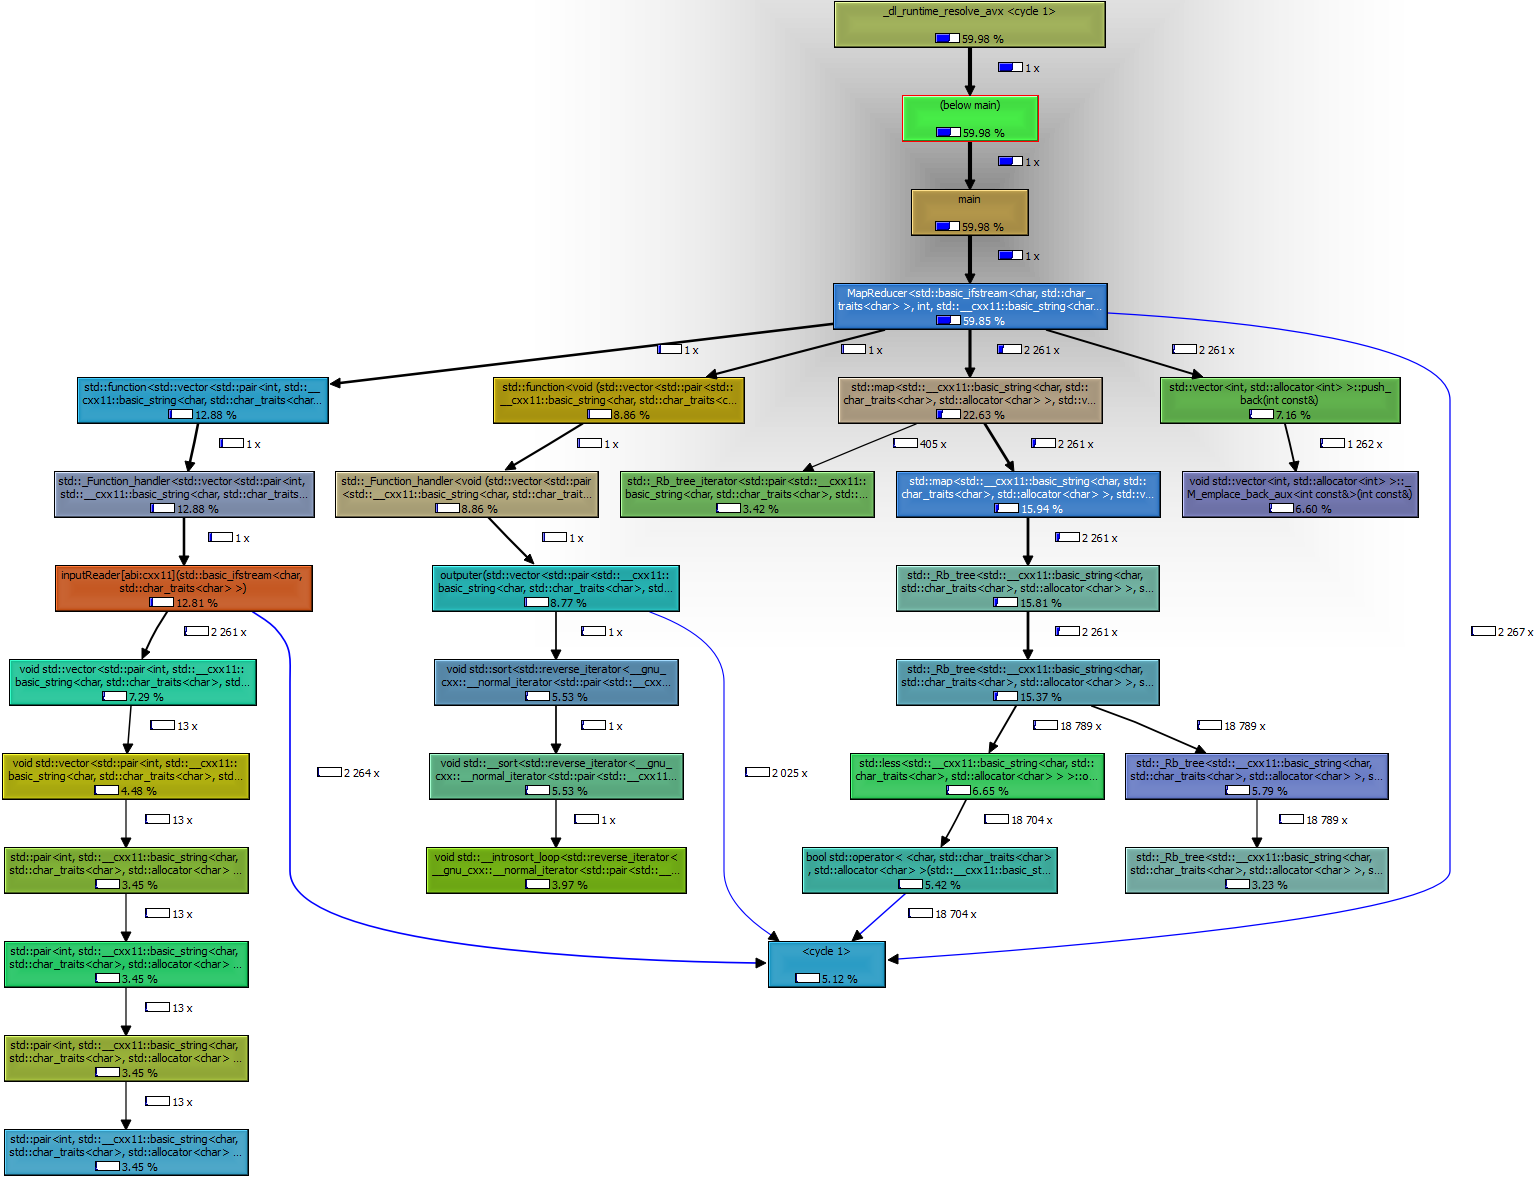
\includegraphics[width=1.35\textwidth, angle=90]{call-graph-part4-cropped}
	\caption{Call map for MapReduce implementation of word count (twelve threads)}
	\end{figure}
\end{document}